\documentclass{standalone}
\usepackage{tikz}
\usetikzlibrary{patterns, positioning}


\begin{document}
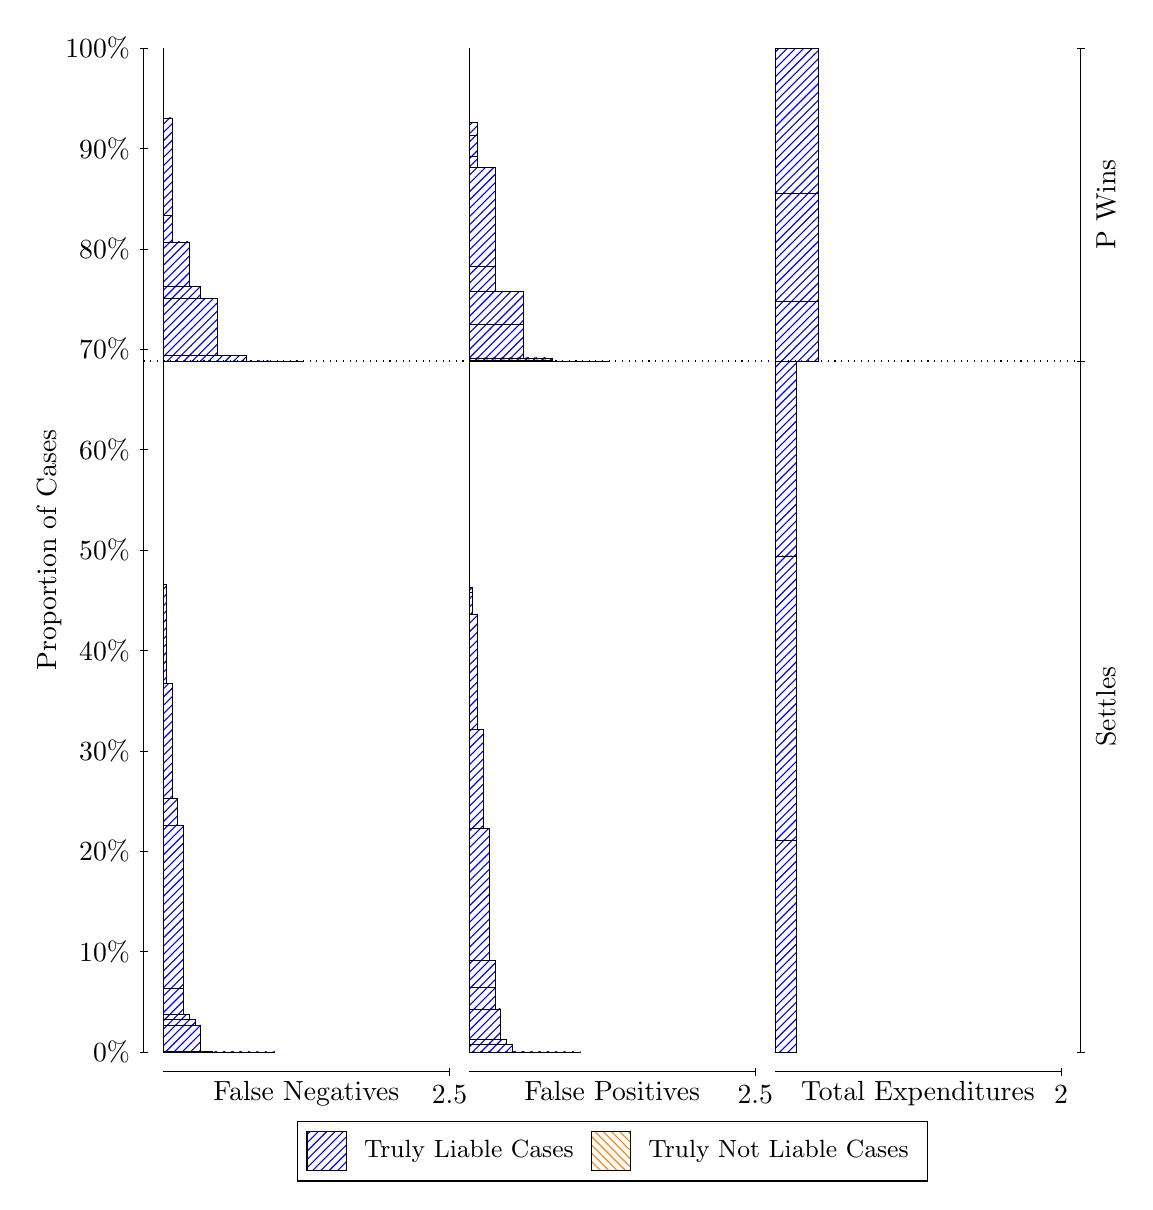
\begin{tikzpicture}
\draw[black, very thin] (1.5,1.75) -- (1.5,14.5);
\node[rotate=90, text=black, anchor=center] at (0.3, 8.125) {Proportion of Cases};
\draw[black, very thin] (1.45,1.75) -- (1.55,1.75);
\node[text=black, anchor=east] at (1.45, 1.75) {0\%};
\draw[black, very thin] (1.45,3.025) -- (1.55,3.025);
\node[text=black, anchor=east] at (1.45, 3.025) {10\%};
\draw[black, very thin] (1.45,4.3) -- (1.55,4.3);
\node[text=black, anchor=east] at (1.45, 4.3) {20\%};
\draw[black, very thin] (1.45,5.575) -- (1.55,5.575);
\node[text=black, anchor=east] at (1.45, 5.575) {30\%};
\draw[black, very thin] (1.45,6.85) -- (1.55,6.85);
\node[text=black, anchor=east] at (1.45, 6.85) {40\%};
\draw[black, very thin] (1.45,8.125) -- (1.55,8.125);
\node[text=black, anchor=east] at (1.45, 8.125) {50\%};
\draw[black, very thin] (1.45,9.4) -- (1.55,9.4);
\node[text=black, anchor=east] at (1.45, 9.4) {60\%};
\draw[black, very thin] (1.45,10.675) -- (1.55,10.675);
\node[text=black, anchor=east] at (1.45, 10.675) {70\%};
\draw[black, very thin] (1.45,11.95) -- (1.55,11.95);
\node[text=black, anchor=east] at (1.45, 11.95) {80\%};
\draw[black, very thin] (1.45,13.225) -- (1.55,13.225);
\node[text=black, anchor=east] at (1.45, 13.225) {90\%};
\draw[black, very thin] (1.45,14.5) -- (1.55,14.5);
\node[text=black, anchor=east] at (1.45, 14.5) {100\%};

\draw[black, very thin] (13.4,1.75) -- (13.4,14.5);
\draw[black, very thin] (13.35,1.75) -- (13.45,1.75);
\node[anchor=west] at (13.35, 1.75) {};
\draw[black, very thin] (13.35,10.525) -- (13.45,10.525);
\node[anchor=west] at (13.35, 10.525) {};
\draw[black, very thin] (13.35,14.5) -- (13.45,14.5);
\node[anchor=west] at (13.35, 14.5) {};

\draw[black, very thin, pattern color=blue, pattern=north east lines] (1.75,1.75) rectangle (3.167,1.75);
\draw[black, very thin, pattern color=blue, pattern=north east lines] (1.75,1.75) rectangle (3.0217,1.75);
\draw[black, very thin, pattern color=blue, pattern=north east lines] (1.75,1.75) rectangle (2.8763,1.75);
\draw[black, very thin, pattern color=blue, pattern=north east lines] (1.75,1.75) rectangle (2.8037,1.75);
\draw[black, very thin, pattern color=blue, pattern=north east lines] (1.75,1.75) rectangle (2.731,1.75);
\draw[black, very thin, pattern color=blue, pattern=north east lines] (1.75,1.75) rectangle (2.6583,1.75);
\draw[black, very thin, pattern color=blue, pattern=north east lines] (1.75,1.75) rectangle (2.5857,1.7508);
\draw[black, very thin, pattern color=blue, pattern=north east lines] (1.75,1.7508) rectangle (2.513,1.7508);
\draw[black, very thin, pattern color=blue, pattern=north east lines] (1.75,1.7508) rectangle (2.4403,1.7508);
\draw[black, very thin, pattern color=blue, pattern=north east lines] (1.75,1.7508) rectangle (2.3677,1.7537);
\draw[black, very thin, pattern color=blue, pattern=north east lines] (1.75,1.7537) rectangle (2.295,1.7575);
\draw[black, very thin, pattern color=blue, pattern=north east lines] (1.75,1.7575) rectangle (2.2223,2.0954);
\draw[black, very thin, pattern color=blue, pattern=north east lines] (1.75,2.0954) rectangle (2.1497,2.1614);
\draw[black, very thin, pattern color=blue, pattern=north east lines] (1.75,2.1614) rectangle (2.077,2.2252);
\draw[black, very thin, pattern color=blue, pattern=north east lines] (1.75,2.2252) rectangle (2.0043,2.5622);
\draw[black, very thin, pattern color=blue, pattern=north east lines] (1.75,2.5622) rectangle (2.0043,4.6279);
\draw[black, very thin, pattern color=blue, pattern=north east lines] (1.75,4.6279) rectangle (1.9317,4.9658);
\draw[black, very thin, pattern color=blue, pattern=north east lines] (1.75,4.9658) rectangle (1.859,6.4281);
\draw[black, very thin, pattern color=blue, pattern=north east lines] (1.75,6.4281) rectangle (1.7863,7.6837);
\draw[black, very thin, pattern color=orange, pattern=north west lines] (1.75,7.6837) rectangle (1.75,7.6837);
\draw[black, very thin, pattern color=blue, pattern=north east lines] (1.75,7.6837) rectangle (1.75,10.525);
\draw[black, very thin, pattern color=blue, pattern=north east lines] (1.75,10.525) rectangle (3.5303,10.525);
\draw[black, very thin, pattern color=blue, pattern=north east lines] (1.75,10.525) rectangle (3.167,10.526);
\draw[black, very thin, pattern color=blue, pattern=north east lines] (1.75,10.526) rectangle (2.949,10.526);
\draw[black, very thin, pattern color=blue, pattern=north east lines] (1.75,10.526) rectangle (2.8037,10.597);
\draw[black, very thin, pattern color=blue, pattern=north east lines] (1.75,10.597) rectangle (2.5857,10.597);
\draw[black, very thin, pattern color=blue, pattern=north east lines] (1.75,10.597) rectangle (2.4403,11.321);
\draw[black, very thin, pattern color=blue, pattern=north east lines] (1.75,11.321) rectangle (2.2223,11.323);
\draw[black, very thin, pattern color=blue, pattern=north east lines] (1.75,11.323) rectangle (2.2223,11.47);
\draw[black, very thin, pattern color=blue, pattern=north east lines] (1.75,11.47) rectangle (2.077,12.038);
\draw[black, very thin, pattern color=blue, pattern=north east lines] (1.75,12.038) rectangle (1.859,12.379);
\draw[black, very thin, pattern color=blue, pattern=north east lines] (1.75,12.379) rectangle (1.859,13.612);
\draw[black, very thin, pattern color=orange, pattern=north west lines] (1.75,13.612) rectangle (1.75,13.612);
\draw[black, very thin, pattern color=blue, pattern=north east lines] (1.75,13.612) rectangle (1.75,14.5);
\draw[black, very thin, pattern color=orange, pattern=north west lines] (5.6333,1.75) rectangle (7.0503,1.75);
\draw[black, very thin, pattern color=blue, pattern=north east lines] (5.6333,1.75) rectangle (7.0503,1.75);
\draw[black, very thin, pattern color=orange, pattern=north west lines] (5.6333,1.75) rectangle (6.7597,1.75);
\draw[black, very thin, pattern color=blue, pattern=north east lines] (5.6333,1.75) rectangle (6.7597,1.75);
\draw[black, very thin, pattern color=blue, pattern=north east lines] (5.6333,1.75) rectangle (6.687,1.75);
\draw[black, very thin, pattern color=orange, pattern=north west lines] (5.6333,1.75) rectangle (6.6143,1.75);
\draw[black, very thin, pattern color=blue, pattern=north east lines] (5.6333,1.75) rectangle (6.6143,1.75);
\draw[black, very thin, pattern color=orange, pattern=north west lines] (5.6333,1.75) rectangle (6.469,1.75);
\draw[black, very thin, pattern color=blue, pattern=north east lines] (5.6333,1.75) rectangle (6.469,1.75);
\draw[black, very thin, pattern color=blue, pattern=north east lines] (5.6333,1.75) rectangle (6.3963,1.75);
\draw[black, very thin, pattern color=orange, pattern=north west lines] (5.6333,1.75) rectangle (6.3237,1.75);
\draw[black, very thin, pattern color=blue, pattern=north east lines] (5.6333,1.75) rectangle (6.3237,1.7508);
\draw[black, very thin, pattern color=blue, pattern=north east lines] (5.6333,1.7508) rectangle (6.3237,1.7513);
\draw[black, very thin, pattern color=blue, pattern=north east lines] (5.6333,1.7513) rectangle (6.251,1.7513);
\draw[black, very thin, pattern color=orange, pattern=north west lines] (5.6333,1.7513) rectangle (6.1783,1.7513);
\draw[black, very thin, pattern color=blue, pattern=north east lines] (5.6333,1.7513) rectangle (6.1783,1.8438);
\draw[black, very thin, pattern color=blue, pattern=north east lines] (5.6333,1.8438) rectangle (6.1057,1.9076);
\draw[black, very thin, pattern color=orange, pattern=north west lines] (5.6333,1.9076) rectangle (6.033,1.9076);
\draw[black, very thin, pattern color=blue, pattern=north east lines] (5.6333,1.9076) rectangle (6.033,2.2945);
\draw[black, very thin, pattern color=blue, pattern=north east lines] (5.6333,2.2945) rectangle (6.033,2.2968);
\draw[black, very thin, pattern color=blue, pattern=north east lines] (5.6333,2.2968) rectangle (5.9603,2.5738);
\draw[black, very thin, pattern color=blue, pattern=north east lines] (5.6333,2.5738) rectangle (5.9603,2.9116);
\draw[black, very thin, pattern color=orange, pattern=north west lines] (5.6333,2.9116) rectangle (5.8877,2.9116);
\draw[black, very thin, pattern color=blue, pattern=north east lines] (5.6333,2.9116) rectangle (5.8877,4.5906);
\draw[black, very thin, pattern color=blue, pattern=north east lines] (5.6333,4.5906) rectangle (5.8877,4.5911);
\draw[black, very thin, pattern color=blue, pattern=north east lines] (5.6333,4.5911) rectangle (5.815,5.8466);
\draw[black, very thin, pattern color=blue, pattern=north east lines] (5.6333,5.8466) rectangle (5.7423,7.309);
\draw[black, very thin, pattern color=blue, pattern=north east lines] (5.6333,7.309) rectangle (5.6697,7.5835);
\draw[black, very thin, pattern color=blue, pattern=north east lines] (5.6333,7.5835) rectangle (5.6697,7.6468);
\draw[black, very thin, pattern color=blue, pattern=north east lines] (5.6333,7.6468) rectangle (5.6333,10.525);
\draw[black, very thin, pattern color=orange, pattern=north west lines] (5.6333,10.525) rectangle (7.4137,10.525);
\draw[black, very thin, pattern color=blue, pattern=north east lines] (5.6333,10.525) rectangle (7.4137,10.525);
\draw[black, very thin, pattern color=blue, pattern=north east lines] (5.6333,10.525) rectangle (7.0503,10.525);
\draw[black, very thin, pattern color=orange, pattern=north west lines] (5.6333,10.525) rectangle (7.0503,10.525);
\draw[black, very thin, pattern color=blue, pattern=north east lines] (5.6333,10.525) rectangle (7.0503,10.525);
\draw[black, very thin, pattern color=blue, pattern=north east lines] (5.6333,10.525) rectangle (6.687,10.54);
\draw[black, very thin, pattern color=orange, pattern=north west lines] (5.6333,10.54) rectangle (6.687,10.54);
\draw[black, very thin, pattern color=blue, pattern=north east lines] (5.6333,10.54) rectangle (6.687,10.566);
\draw[black, very thin, pattern color=orange, pattern=north west lines] (5.6333,10.566) rectangle (6.469,10.566);
\draw[black, very thin, pattern color=blue, pattern=north east lines] (5.6333,10.566) rectangle (6.469,10.566);
\draw[black, very thin, pattern color=blue, pattern=north east lines] (5.6333,10.566) rectangle (6.3237,10.991);
\draw[black, very thin, pattern color=orange, pattern=north west lines] (5.6333,10.991) rectangle (6.3237,10.991);
\draw[black, very thin, pattern color=blue, pattern=north east lines] (5.6333,10.991) rectangle (6.3237,11.412);
\draw[black, very thin, pattern color=orange, pattern=north west lines] (5.6333,11.412) rectangle (6.1057,11.412);
\draw[black, very thin, pattern color=blue, pattern=north east lines] (5.6333,11.412) rectangle (6.1057,11.412);
\draw[black, very thin, pattern color=blue, pattern=north east lines] (5.6333,11.412) rectangle (6.1057,11.413);
\draw[black, very thin, pattern color=blue, pattern=north east lines] (5.6333,11.413) rectangle (5.9603,11.731);
\draw[black, very thin, pattern color=blue, pattern=north east lines] (5.6333,11.731) rectangle (5.9603,12.986);
\draw[black, very thin, pattern color=blue, pattern=north east lines] (5.6333,12.986) rectangle (5.7423,13.127);
\draw[black, very thin, pattern color=orange, pattern=north west lines] (5.6333,13.127) rectangle (5.7423,13.127);
\draw[black, very thin, pattern color=blue, pattern=north east lines] (5.6333,13.127) rectangle (5.7423,13.386);
\draw[black, very thin, pattern color=blue, pattern=north east lines] (5.6333,13.386) rectangle (5.7423,13.554);
\draw[black, very thin, pattern color=blue, pattern=north east lines] (5.6333,13.554) rectangle (5.6333,14.5);
\draw[black, very thin, pattern color=orange, pattern=north west lines] (9.5167,1.75) rectangle (9.7892,1.75);
\draw[black, very thin, pattern color=blue, pattern=north east lines] (9.5167,1.75) rectangle (9.7892,4.4435);
\draw[black, very thin, pattern color=orange, pattern=north west lines] (9.5167,4.4435) rectangle (9.7892,4.4435);
\draw[black, very thin, pattern color=blue, pattern=north east lines] (9.5167,4.4435) rectangle (9.7892,8.0506);
\draw[black, very thin, pattern color=orange, pattern=north west lines] (9.5167,8.0506) rectangle (9.7892,8.0506);
\draw[black, very thin, pattern color=blue, pattern=north east lines] (9.5167,8.0506) rectangle (9.7892,10.525);
\draw[black, very thin, pattern color=orange, pattern=north west lines] (9.5167,10.525) rectangle (10.062,10.525);
\draw[black, very thin, pattern color=blue, pattern=north east lines] (9.5167,10.525) rectangle (10.062,11.283);
\draw[black, very thin, pattern color=orange, pattern=north west lines] (9.5167,11.283) rectangle (10.062,11.283);
\draw[black, very thin, pattern color=blue, pattern=north east lines] (9.5167,11.283) rectangle (10.062,12.659);
\draw[black, very thin, pattern color=orange, pattern=north west lines] (9.5167,12.659) rectangle (10.062,12.659);
\draw[black, very thin, pattern color=blue, pattern=north east lines] (9.5167,12.659) rectangle (10.062,14.5);
\draw[black, dotted] (1.5,10.525) -- (13.4,10.525);
\draw[black, very thin] (1.75,1.5) -- (5.3833,1.5);
\node[text=black, anchor=north] at (3.5667, 1.5) {False Negatives};
\draw[black, very thin] (5.3833,1.45) -- (5.3833,1.55);
\node[text=black, anchor=north] at (5.3833, 1.45) {2.5};

\draw[black, very thin] (5.6333,1.5) -- (9.2667,1.5);
\node[text=black, anchor=north] at (7.45, 1.5) {False Positives};
\draw[black, very thin] (9.2667,1.45) -- (9.2667,1.55);
\node[text=black, anchor=north] at (9.2667, 1.45) {2.5};

\draw[black, very thin] (9.5167,1.5) -- (13.15,1.5);
\node[text=black, anchor=north] at (11.333, 1.5) {Total Expenditures};
\draw[black, very thin] (13.15,1.45) -- (13.15,1.55);
\node[text=black, anchor=north] at (13.15, 1.45) {2};

\node[text=black, centered, rotate=90] at (13.72, 6.1374) {Settles};
\node[text=black, centered, rotate=90] at (13.72, 12.512) {P Wins};

\draw (7.449999999999999,1.5) node[draw=none] (baseCoordinate) {};
\begin{scope}[align=center]
        \matrix[scale=0.5, draw=black, below=0.5cm of baseCoordinate, nodes={draw}, column sep=0.1cm]{
            \node[rectangle, draw, minimum width=0.5cm, minimum height=0.5cm, pattern color=blue, pattern=north east lines] {}; &
            \node[draw=none, font=\small, text=black] (B) {Truly Liable Cases}; &
            \node[rectangle, draw, minimum width=0.5cm, minimum height=0.5cm, pattern color=orange, pattern=north west lines] {}; &
            \node[draw=none, font=\small, text=black] (B) {Truly Not Liable Cases}; \\
            };
\end{scope}

\end{tikzpicture}
\end{document}